\chapter{Instructieselectie}

De meeste architecturen hebben complexere instructies dan degene die in de IR tree gegeven zijn. Bijna elke architectuur kan een add en een fetch uitvoeren in één enkele instructie. 
\section{Boompatronen}
Een machine-instructie is een fragment van de IR tree. Deze fragmenten worden \textbf{boompatronen} genoemd. Instructieselectie is dan het proces om de IR tree te bedekken met een minimaal aantal patronen.

\begin{figure}
	\centering
	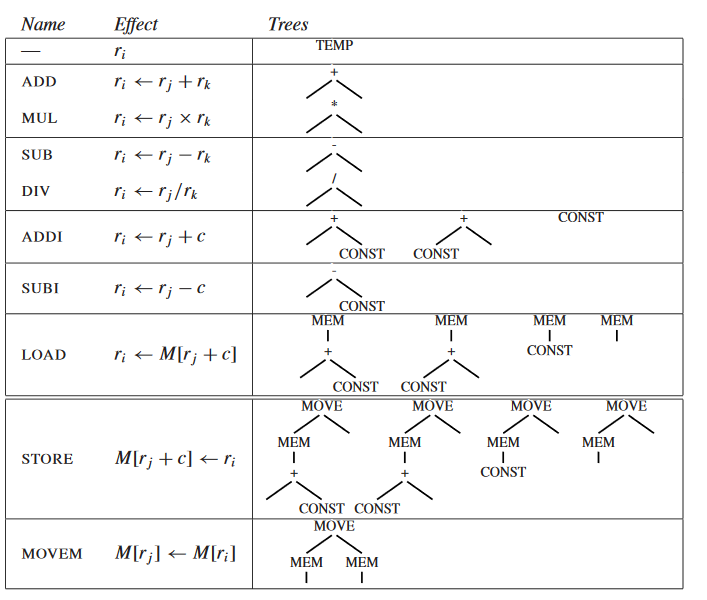
\includegraphics[width=0.7\textwidth]{jouette_instructions}
	\caption{Geheugen -en rekenoperaties. De notatie M[x] geeft het processorwoord op adress x.}
	\label{fig:jouette_instructions}
\end{figure}

Figuur \ref{fig:jouette_instructions} toont de instructieset van een \textit{uitgevonden} architectuur, \textbf{Jouette}. Elke instructie boven de dubbele lijn genereert een waarde in een register. De instructies onder de dubbele lijn bewaren niets in het register. Elke instructie heeft één of meerdere boompatronen.

Nu moet een IR tree bedekt worden met deze boompatronen. Dit heet ook \textbf{tiling} en geen enkele tile mag overlappen. Op figuur \ref{fig:tree_tiling} worden twee bomen, die identiek zijn, op een andere manier bedekt. 

\begin{figure}
	\centering
	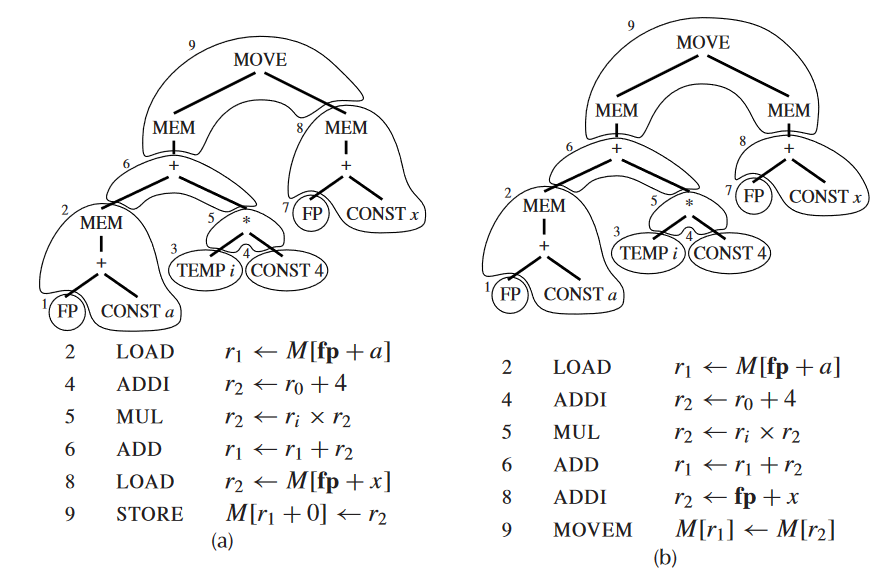
\includegraphics[width=0.7\textwidth]{tree_tiling}
	\caption{Een boom kan op meerdere manieren bedekt worden.}
	\label{fig:tree_tiling}
\end{figure}
De beste bedekking is degene die het minst 'kost'. Enerzijds kan dit het aantal instructies zijn en anderzijds de tijd die één instructie in beslag neemt. Een \textbf{optimale bedekking} wordt gedefinieerd als de bedekking waarbij:
\begin{enumerate}
	\item \textbf{optimum criterium}: de totale kost minimaal is;
	\item \textbf{optimaal criterium}: twee aaneensluitende tiles niet gecombineerd kunnen worden tot één tile met lagere kost.
\end{enumerate}
Wanneer het optimum criteria voldaan wordt, is het optimaal criteria ook automatisch voldaan. Andersom geldt het niet.

\section{Algoritmen voor instructieselectie}
\begin{table}[ht]
	\centering
	\begin{tabular}{l | l}
		RISC & CISC \\
		32 registers & weining registers \\
		Register-register architectuur & Memory-memory architectuur \\
		3-adresinstructies: R1 $\rightarrow$ R2 op R3 & 2-adresinstructies: R1 $\rightarrow$ R1 op R2 \\
		1 adresseermode & veel adresseermodes \\
		Vaste instructielengte & variabele instructielengte \\
	\end{tabular}
\end{table}

\subsection{Maximal Munch}
Het algoritme voor optimale bedekking heet \textbf{Maximal Munch}:
\begin{enumerate}
	\item Begin bij de wortel van de boom en zoek de grootste tile dat past. De grootste tile is degene met het meest knopen. Als er meerdere tiles zijn met hetzelfde aantal knopen, wordt er random gekozen.
	\item Bedek de wortel, en eventueel andere knopen, met deze tile.
	\item Er onstaan nu deelbomen, waarop hetzelfde principe kan toegepast worden.
\end{enumerate}

\subsection{Dynamisch programmeren}
De optimale bedekking is NP-compleet. Het Maximal Munch algoritme zal altijd aan het optimaal criterium voldoen, maar niet aan het optimum criterium. Om het optimum criterium toch te laten voldoen, wordt dynamisch programmeren gebruikt. In deze versie krijgt elke knoop een kost die gelijk is aan de som van de laagste instructiekosten van de deelboom waarvan de knoop wortel is, bedekt kan worden. Het algoritme loopt nu als volgt:
\begin{enumerate}
	\item Bereken de kost van elke knoop bottom-up. De kost van een knoop $n$ wordt bepaald door eerst de kost van zijn kinderen, kleinkinderen, enz... te bepalen. 
	\item Elke tile wordt nu gematched tegen node $n$. Voor elke tile $t$ met kost $c$ that op $n$ gelegd kan worden zullen er nul of meer deelbomen $d_i$ zijn die overeenkomen met de bladeren van deze tiles. Een blad van een tile zijn knopen waaraan een deelboom kan aangehangen worden. De kost $c_i$ van elke deelboom is reeds gekend, dus de kost van tile $t$ is $c + \sum c_i$.
	\item Voor elke tile $t_j$ dat $n$ kan bedekken, diegene met de minimale kost wordt gekozen.
\end{enumerate}
